\documentclass[11pt, a4paper]{article}

\pdfminorversion=7

\usepackage[utf8]{inputenc} % Input encoding (allows æ, ø, å  fx)
\usepackage[T1]{fontenc} % Font encoding
\usepackage[backend=biber]{biblatex} % source tool
\usepackage[a4paper]{geometry} % Layout (margins, page size)
\usepackage{inconsolata} % Monospace font
\usepackage{charter} % Font family
\usepackage[outputdir=build]{minted} % Code highlight
\usepackage{booktabs} % beautiful tables
\usepackage{float} % force positioning of figures
\usepackage[labelfont=bf, textfont=it]{caption} % control figure and table captions
\usepackage{graphicx} % insert graphics
\usepackage{fancyhdr} % page header (and footer)
\usepackage[titletoc]{appendix} % ... appendix
\usepackage{minitoc} % table of contents stuff
\usepackage[hidelinks=true, hypertexnames=false]{hyperref} % references in text (and clickable links)

\graphicspath{ {./images/} }
\addbibresource{sources.bib}

\newcommand{\tmp}[1]{{\color{red}#1}}
\newcommand{\inlinecode}[1]{\texttt{#1}}
\newcommand{\appendixref}[1]{\hyperref[#1]{Appendix~\ref{#1}}}

\renewcommand{\baselinestretch}{1.2} % Line spacing
\setlength{\parindent}{0em} % Paragraph indent
\setlength{\parskip}{0.75em} % Paragraph vertical spacing
\setlength\headheight{14pt}

\setcounter{tocdepth}{3} % How deep the table of contents goes

\renewcommand*{\nameyeardelim}{\addcomma\space}

% Make the "Part I" text invisible
\renewcommand \thepart{}
\renewcommand \partname{}

\begin{document}
    \begin{titlepage}
        \newcommand{\HRule}{\rule{1.25\linewidth}{0.5mm}}
\center
\vspace*{-4.35cm}
\makebox[\textwidth][c]{
\includegraphics[width=1\paperwidth]{devops-banner.pdf}}%
% \ \\[1cm]
% \hbox{\makebox[1\textwidth][c]{\textsc{\Large Course: \textit{DevOps, Software Evolution and Software Maintenance}}}}
\vspace{3cm}
\textsc{\large Course code: BSDSESM1KU}
\\[0.2cm]
\textsc{\large Bachelor in Software Development}
\\[0.5cm]
\hbox{\makebox[1\textwidth][c]{\HRule}}
\vspace{0.4cm}
{ \huge \bfseries DevOps: ITU-MiniTwit}
\\[0.6cm]
\hbox{\makebox[1\textwidth][c]{\HRule}}
\vspace{0.9cm}
\textsc{\Large Group R --- Rhododevdron\\[0.5cm]IT University of Copenhagen}\\[1.5cm]
\begin{tabular}{ll}
\toprule
\textbf{Name} & \textbf{Email} \\
\midrule
Adrian Valdemar Borup & adbo@itu.dk \\
Albert Rise Nielsen & albn@itu.dk \\
Joachim Alexander Borup & aljb@itu.dk \\
Thomas Wolgast Rørbech & thwr@itu.dk \\
\bottomrule
\end{tabular}
\\[2cm]
{\large \today}
\\[1.5cm]
{\large 3455 words}
\vfill

    \end{titlepage}
    \newgeometry{left=2.54cm, right=2.54cm, top=2.54cm, bottom=2.54cm}
    \pagestyle{fancy}
    \fancyhf{}
    \rhead{Group R, BSDSESM1KU}
    \chead{\today}
    \lhead{IT University of Copenhagen}
    \cfoot{\thepage\ of \pageref{page:lastpage}}

    \doparttoc % Tell to minitoc to generate a toc for the parts
    \noptcrule
    \bgroup
    \setcounter{parttocdepth}{5}
    \renewcommand\baselinestretch{1}
    \setlength{\parskip}{0.1em}
    \faketableofcontents % Run a fake tableofcontents command for the partocs
    \part{} % Start the document part
    \parttoc % Insert the document TOC
    \egroup
    \newpage

    \section{System Perspective}
\subsection{Software license compatibility}
To check if the software licenses of the libraries we've used are compatible with the MIT license in our repository, we have used lichen \cite{tool:lichen} to automatically check the licenses of all used libraries. This process is documented in \appendixref{appendix:software-license-check}. The results showed that all the libraries were compatible, except one because the tool couldn't find its license. However, checking its repository manually revealed a compatible MIT license.

\subsection{System dependencies}
\autoref{table:system-dependencies} shows most of the major tools, libraries, and other technologies our systems depend on.
\begin{table}[H]
    \makebox[\textwidth][c]{
        \bgroup
        \renewcommand{\arraystretch}{1.2}
        \begin{tabular}{p{0.235\linewidth} | p{0.375\linewidth} | p{0.5\linewidth}}
            \toprule
            \textbf{Category} & \textbf{Tools and technologies} & \textbf{Description} \\
            \midrule

            \textbf{Version control} & Git~\cite{tool:git}, GitHub~\cite{tool:github} & Source code accessible for all developers, tracking issues, creating notes and tasks. \\
            \textbf{Pipeline CI/CD} & CircleCi~\cite{tool:circleci} & Automate task such as; testing, building, deploying, releasing, generating changelog. \\
            \textbf{Containerization} & Docker~\cite{tool:docker}, DockerHub~\cite{tool:docker-hub} & Ensure same development environment and deployment to DockerHub. \\

            \textbf{Infrastructure} & Terraform~\cite{tool:terraform} & IaC, Make it easier to swap host, automate tasks for releases. \\
            \textbf{Service provider} & Azure~\cite{tool:azure}, own server~\cite{tool:kubeadm} & Hosting our app. \\
            \textbf{Service management} & Kubernetes~\cite{tool:kubernetes} & Orchestrate containers, scaling up / down, load balancing. \\
            \textbf{Database} & SQL Server~\cite{tool:microsoft-sql-server}, SQLite~\cite{tool:sql-lite} & To store user data. \\

            \textbf{Logging} & Elasticsearch~\cite{tool:elasticsearch}, Fluentd~\cite{tool:fluentd}, Kibana~\cite{tool:kibana} & To gather logs into a centralized log and sort, filter, search the centralized log. \\
            \textbf{Monitoring} & Grafana~\cite{tool:grafana}, Prometheus~\cite{tool:prometheus} & Gather and organize metrics from our system, based on those create alerts and a visual representation. \\

            \textbf{Languages} & Golang~\cite{tool:go}, TypeScript~\cite{tool:typescript} & Backend and frontend. \\ 
            \textbf{Frameworks} & GORM~\cite{gorm}, testify~\cite{tool:testify}, gin-gonic~\cite{tool:gin}, VueJS~\cite{tool:vue} & ORM, Testing, HTTP Framework, Frontend SPA. \\
            \textbf{Code analysis} & SonarCloud~\cite{tool:sonarcloud}, Better Code Hub~\cite{tool:bettercodehub}, lint~\cite{tool:golang-lint} cyclomatic~\cite{tool:go-cyclo} & Increase code quality and motivate clean code. \\
            \textbf{Security} & Snyk~\cite{snyk}, OWASP Zap~\cite{tool:owasp-zap}, Metasploit~\cite{metasploit} WMAP~\cite{metasploit-wmap} & Notify about Security issues and updates to dependencies and scan for vulnerabilities. \\

            \textbf{Documentation} & LaTeX~\cite{tool:latex}, Markdown~\cite{tool:markdown} & Report, notes, changelog, instructions. \\
            \bottomrule
        \end{tabular}
        \egroup
    }
    \caption{The tools and technologies that our system depends on.}
    \label{table:system-dependencies}
\end{table}


    \section{Process Perspective}

\subsection{Team interaction}

The team consists of 4 developers, who meet once or twice a week to work on the project. At each meeting, the developers discuss the tasks at hand, create issues, divide the work, and then spends the rest of the time working on their tasks. There is no hierarchy - only 4 like-minded developers who makes decisions in unison.

New tasks are created as issues on GitHub, and then assigned to the developer who will be working on it. Maintaining a set of issues on GitHub lets us keep an overview of the planned tasks, and allows for any of the developers to easily add a new task at any time.

\subsection{Organisation of repositories}
The group uses GitHub to manage repositories. On GitHub, we have a dedicated organization that owns all of the project repositories. This way, we can keep related repositories together and reuse permission settings on GitHub. Currently, we have the following repositories:
\begin{enumerate}
  \item \href{https://github.com/Devops-2022-Group-R/itu-minitwit}{\inlinecode{Devops-2022-Group-R/itu-minitwit}}, which is the main project repository. Here, we have the backend web server which handles all business logic.
  \item \href{https://github.com/Devops-2022-Group-R/itu-minitwit-frontend}{\inlinecode{Devops-2022-Group-R/itu-minitwit-frontend}}, containing our frontend web-app.
  \item \href{https://github.com/Devops-2022-Group-R/flag-tool}{\inlinecode{Devops-2022-Group-R/flag-tool}}, which is a rewrite of the original flag tool given with the project template. The tool has been rewritten and moved to a separate repository.
  \item \href{https://github.com/Devops-2022-Group-R/bump-tool}{\inlinecode{Devops-2022-Group-R/bump-tool}}, which is a small tool to help with finding the next version bump based on a pull request's tag (major/minor/patch) and the project's current version.
\end{enumerate}
The general philosophy has been to separate parts that can exist alone with a single responsibility. This way, all issues, pull requests, and releases are related to the topic of the repository. In a monolithic repository, you have to put in more effort to specify which part of the repository is relevant for a PR or issue. This also allows for easier and more simple CI/CD pipelines, and it becomes more obvious what a release changes. One example of this separation is the frontend web application, which is completely separated from the backend, with Kubernetes specs and CI/CD pipelines in its own repository.

However, we've not been as good at following this philosophy as we would like to. For example, our monitoring is a separate entity from our web server, but all the monitoring configuration is stored in the \inlinecode{itu-minitwit} repository \cite{repo:monitoring-config} \cite{repo:monitoring-kubernetes}. Instead, we should have moved this to a separate repository because it does not have anything to do with how the web server operates.

The same goes for the LaTeX files that this report consists of. We would have liked to have a separate repository for this to keep Git history clean and CI/CD more separate, but in this case it is a project requirement to have it in the main repository.

\subsection{Git branching strategy}
We have applied trunk-based development, meaning we branch out from the main branch, have a branch that lives shortly until the changes are implemented, and then merge it directly into the main branch. This keeps unrelated changes separate and makes PRs easier to review and merge. It's worth noting that we do not utilise release branches from trunk-based development, because we release continuously for each merge into the main branch.

\subsection{Monitoring}
To monitor our systems, Prometheus is used to collect metrics and Grafana is used to visualize them. We chose to monitor the number of requests and request latency for each endpoint on our server, and we monitored the CPU and memory usage of it. We chose these because they give a quick overview of how the system is performing. The remaining information is stored in our logs.

For an example where we had an issue with our system, which was reflected in the monitoring, see \appendixref{appendix:monitoring-samples}.

\begin{figure}[H]
    \makebox[\textwidth][c]{
        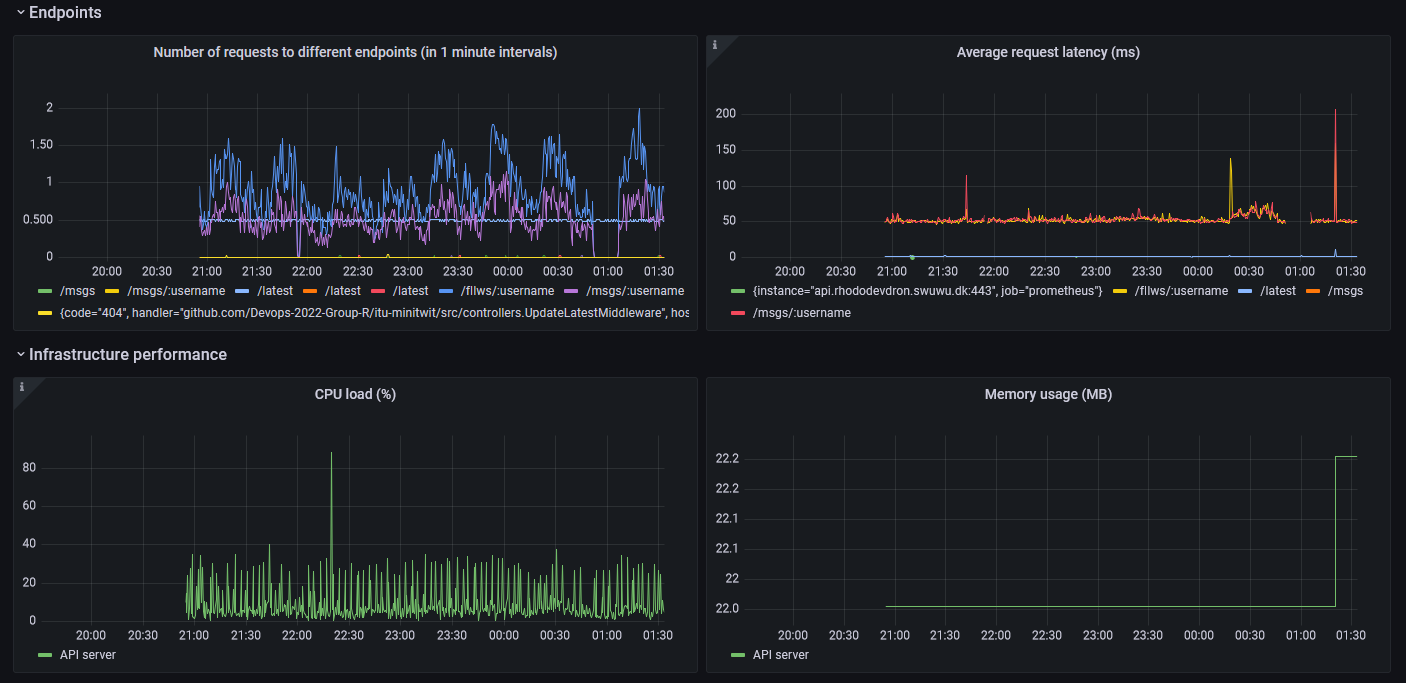
\includegraphics[width=0.85\paperwidth]{grafana-dashboard}
    }%
    \caption{A sample of our Grafana dashboard.}
\end{figure}

\subsection{Logging}
\label{section:process-logging}
We log using JSON, which allows us to select specific fields to display in Kibana, making the logs easy to read, filter, and sort by. \autoref{fig:logs-example} shows how we display logs in an easy-to-read format.
\begin{figure}[H]
  \makebox[\textwidth][c]{
    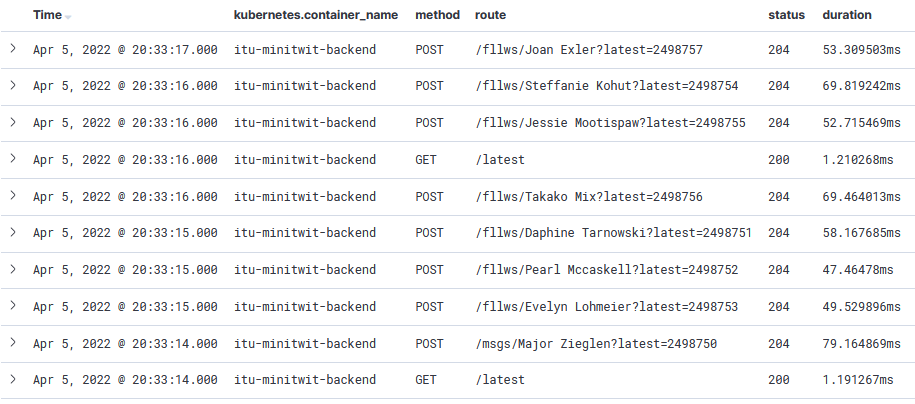
\includegraphics[width=0.9\paperwidth]{kibana-logs-structure.png}
  }
  \caption{Example of how we view logs in Kibana.}
  \label{fig:logs-example}
\end{figure}
It's not shown on the figure, but we also have a column for error messages, which we've experienced makes it easy to diagnose problems in the system. To diagnose performance issues, the ``duration'' column has also been helpful. By the end of the project, the mentioned log output has been enough to diagnose bugs and get an overview of what's happening in the system.

\subsection{Strategy for scaling and load balancing}
We have deployed all of our components with Kubernetes deployments \cite{docs:kubernetes-deployment}, and configured them to run behind Kubernetes services \cite{docs:kubernetes-service}, this ensures component level load balancing.
Using deployments also allows us to manually scale the number of instances of each component. While deployments do have the ability to autoscale, after some configuration, we have decided against it due to cost issues and because our monitoring indicated that the system was not getting enough load to justify scaling.

Deployments also support zero downtime updates. This is achieved by changing settings on the deployment, such as the image to be used, then Kubernetes creates a new pod, and then kills an old pod when the new is ready, repeating the process until all pods have the new configuration.



    \nocite{*}
    \setlength\bibitemsep{1.5\itemsep}
    \printbibliography[heading=bibnumbered]
    \label{page:lastpage}

    \bgroup
\newpage
\cfoot{\thepage}
\setcounter{page}{1}
\pagenumbering{roman}
\topskip0pt
\begin{center}
    \begin{figure}[H]
        \setbox0=\vbox{
         \caption{} % ugly hack to make appendix link in the TOC link to this page
        }
        \addcontentsline{toc}{section}{Appendices} % Add the appendix text to the document TOC
    \end{figure}
    \part{Appendices} % Start the appendix part in TOC
    \renewcommand\baselinestretch{1}
    \setlength{\parskip}{0.1em}
    \parttoc % Insert the appendix TOC
\end{center}
\begin{appendices}
\newpage
\section{Checking software license compatibility}
\label{appendix:software-license-check}
To run the license scan tool, we used:
\begin{minted}{bash}
  # Install
  go install github.com/uw-labs/lichen@latest
  # Run in root of Devops-2022-Group-R/itu-minitwit/
  go build -o my-binary ./src
  lichen my-binary
\end{minted}
This reveals that the only disallowed library we use is \inlinecode{Azure/azure-sdk-for-go/sdk/internal} because it's missing a license. However, if you check the repository manually, you can find a MIT license in the root.

The output of the command is:
\bgroup
\small
\begin{minted}{bash}
github.com/Azure/azure-sdk-for-go/sdk/azcore@v0.19.0: MIT (allowed)
github.com/Azure/azure-sdk-for-go/sdk/azidentity@v0.11.0: MIT (allowed)
github.com/Azure/azure-sdk-for-go/sdk/internal@v0.7.0:  (not allowed - unresolvable license)
github.com/beorn7/perks@v1.0.1: MIT (allowed)
github.com/cespare/xxhash/v2@v2.1.2: MIT (allowed)
github.com/denisenkom/go-mssqldb@v0.12.0: BSD-3-Clause (allowed)
github.com/gin-contrib/sse@v0.1.0: MIT (allowed)
github.com/gin-gonic/gin@v1.7.7: MIT (allowed)
github.com/go-playground/locales@v0.14.0: MIT (allowed)
github.com/go-playground/universal-translator@v0.18.0: MIT (allowed)
github.com/go-playground/validator/v10@v10.10.0: MIT (allowed)
github.com/golang-sql/civil@v0.0.0-20190719163853-cb61b32ac6fe: Apache-2.0 (allowed)
github.com/golang-sql/sqlexp@v0.0.0-20170517235910-f1bb20e5a188: BSD-3-Clause (allowed)
github.com/golang/protobuf@v1.5.2: BSD-3-Clause (allowed)
github.com/jinzhu/inflection@v1.0.0: MIT (allowed)
github.com/jinzhu/now@v1.1.4: MIT (allowed)
github.com/leodido/go-urn@v1.2.1: MIT (allowed)
github.com/mattn/go-isatty@v0.0.14: MIT (allowed)
github.com/mattn/go-sqlite3@v1.14.11: MIT (allowed)
github.com/matttproud/golang_protobuf_extensions@v1.0.1: Apache-2.0 (allowed)
github.com/pkg/browser@v0.0.0-20180916011732-0a3d74bf9ce4: BSD-2-Clause (allowed)
github.com/prometheus/client_golang@v1.12.1: Apache-2.0 (allowed)
github.com/prometheus/client_model@v0.2.0: Apache-2.0 (allowed)
github.com/prometheus/common@v0.32.1: Apache-2.0 (allowed)
github.com/prometheus/procfs@v0.7.3: Apache-2.0 (allowed)
github.com/shirou/gopsutil@v3.21.11+incompatible: BSD-3-Clause (allowed)
github.com/sirupsen/logrus@v1.6.0: MIT (allowed)
github.com/tklauser/go-sysconf@v0.3.10: BSD-3-Clause (allowed)
github.com/tklauser/numcpus@v0.4.0: Apache-2.0 (allowed)
github.com/ugorji/go/codec@v1.2.6: MIT (allowed)
github.com/zsais/go-gin-prometheus@v0.1.0: MIT (allowed)
golang.org/x/crypto@v0.0.0-20220210151621-f4118a5b28e2: BSD-3-Clause (allowed)
golang.org/x/net@v0.0.0-20211112202133-69e39bad7dc2: BSD-3-Clause (allowed)
golang.org/x/sys@v0.0.0-20220209214540-3681064d5158: BSD-3-Clause (allowed)
golang.org/x/text@v0.3.7: BSD-3-Clause (allowed)
google.golang.org/protobuf@v1.27.1: BSD-3-Clause (allowed)
gopkg.in/yaml.v2@v2.4.0: Apache-2.0, MIT (allowed)
gorm.io/driver/sqlite@v1.2.6: MIT (allowed)
gorm.io/driver/sqlserver@v1.3.1: MIT (allowed)
gorm.io/gorm@v1.23.1: MIT (allowed)
2022/03/20 14:23:40 1 error occurred:
      * github.com/Azure/azure-sdk-for-go/sdk/internal@v0.7.0: not allowed - unresolvable
        license
\end{minted}
\egroup

\newpage
\section{Monitoring example: High CPU usage}
\label{appendix:monitoring-samples}
\autoref{fig:grafana-dashboard-cpu} and \autoref{fig:azure-dashboard-cpu} show the status of our system in Grafana and Azure when we tried to implement logging. The initial implementation used up high amounts of our CPU resources, which is reflected in the response times and CPU recording metrics.
\begin{figure}[H]
    \begin{center}
        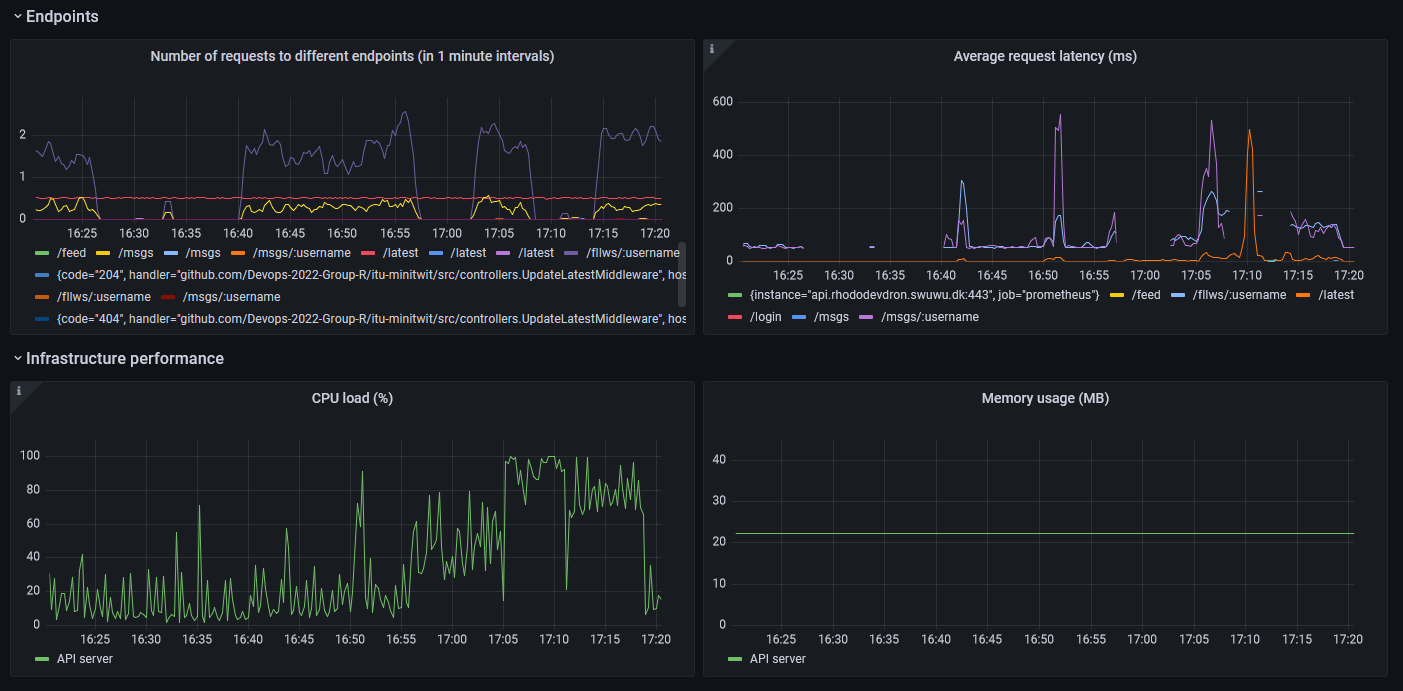
\includegraphics[width=1\textwidth]{grafana-dashboard-cpu.png}
    \end{center}
    \caption{A snapshot of our Grafana monitoring dashboard.}
    \label{fig:grafana-dashboard-cpu}
\end{figure}
\begin{figure}[H]
    \begin{center}
        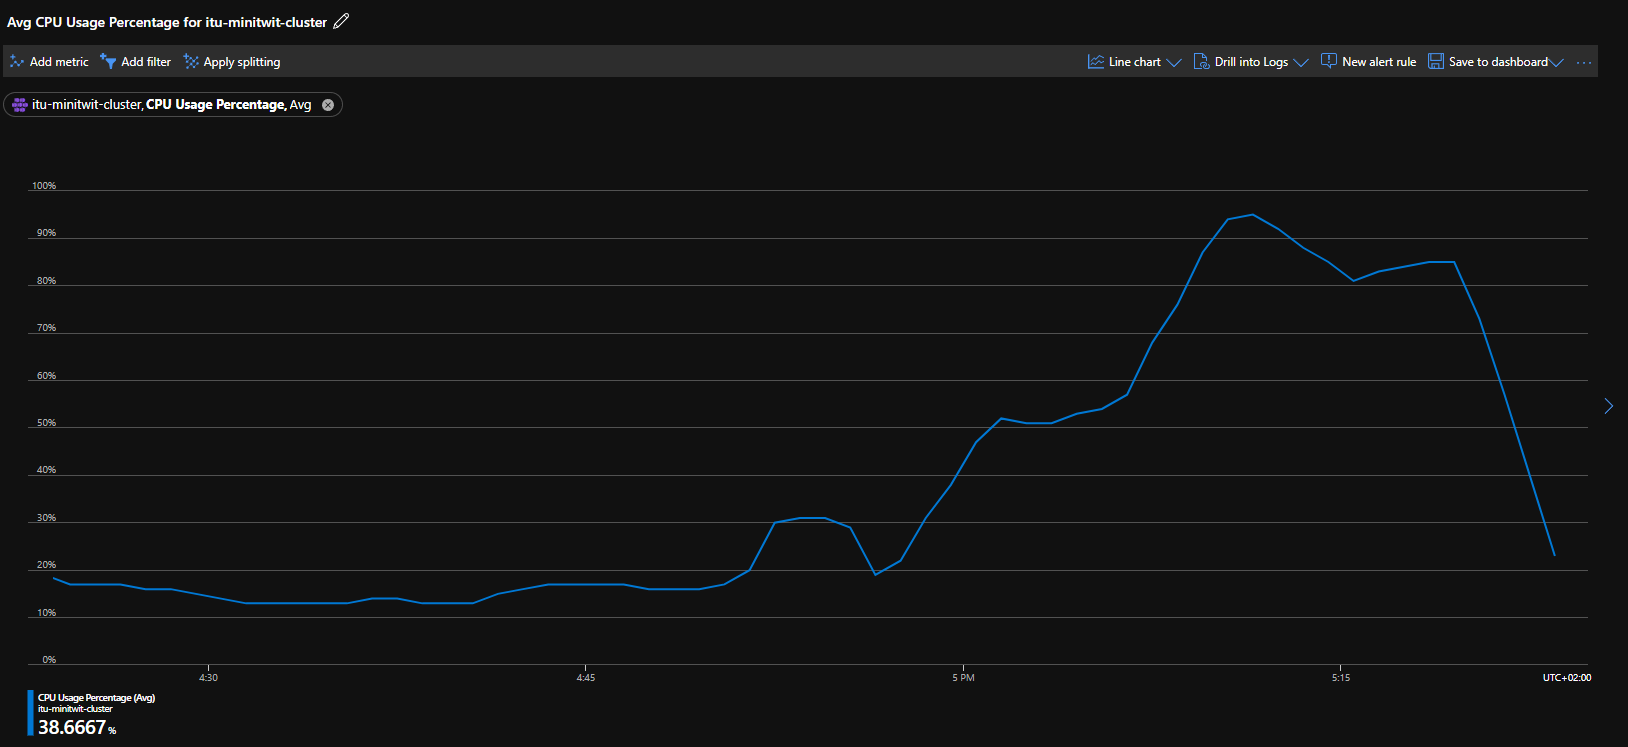
\includegraphics[width=1\textwidth]{azure-dashboard-cpu.png}
    \end{center}
    \caption{A graph from Azure's monitoring showing the CPU usage of our cluster.}
    \label{fig:azure-dashboard-cpu}
\end{figure}

\end{appendices}
\egroup

\end{document}
